%!TEX encoding = UTF-8 Unicode
\documentclass{lecturenotes}

\renewcommand{\vecka}{7}
\newcommand{\veckotema}{Mängder, tabeller}

%!TEX encoding = UTF-8 Unicode
\setbeamertemplate{footline}[frame number]

\newcommand{\LibVersion}{0.1.0} % latest version of introlib at https://github.com/lunduniversity/introprog-scalalib
\newcommand{\LibJar}{\texttt{introprog-\LibVersion.jar}}
\newcommand{\JDKApiUrl}{\url{https://docs.oracle.com/javase/8/docs/api/}}


\title[Föreläsningsanteckningar EDAA45, \CurrentYear]{EDAA45 Programmering, grundkurs}
\subtitle{Läsvecka \vecka: \veckotema}
\author{Björn Regnell}
\institute{Datavetenskap, LTH}
\date{Lp1-2, HT \CurrentYear}

%!TEX encoding = UTF-8 Unicode

\newcommand{\ModWeekONE}{Introduktion}
\newcommand{\ExeWeekONE}{expressions}
\newcommand{\LabWeekONE}{kojo}


\newcommand{\ModWeekTWO}{Program, kontrollstrukturer}
\newcommand{\ExeWeekTWO}{programs}
\newcommand{\LabWeekTWO}{--}


\newcommand{\ModWeekTHREE}{Funktioner, abstraktion}
\newcommand{\ExeWeekTHREE}{functions}
\newcommand{\LabWeekTHREE}{irritext}


\newcommand{\ModWeekFOUR}{Objekt, inkapsling}
\newcommand{\ExeWeekFOUR}{objects}
\newcommand{\LabWeekFOUR}{blockmole}


\newcommand{\ModWeekFIVE}{Klasser, datamodellering}
\newcommand{\ExeWeekFIVE}{classes}
\newcommand{\LabWeekFIVE}{--}


\newcommand{\ModWeekSIX}{Mönster, felhantering}
\newcommand{\ExeWeekSIX}{patterns}
\newcommand{\LabWeekSIX}{blockbattle}


\newcommand{\ModWeekSEVEN}{Sekvenser, enumerationer}
\newcommand{\ExeWeekSEVEN}{sequences}
\newcommand{\LabWeekSEVEN}{shuffle}


\newcommand{\ModWeekEIGHT}{Matriser, typparametrar}
\newcommand{\ExeWeekEIGHT}{matrices}
\newcommand{\LabWeekEIGHT}{life}


\newcommand{\ModWeekNINE}{Mängder, tabeller}
\newcommand{\ExeWeekNINE}{lookup}
\newcommand{\LabWeekNINE}{words}


\newcommand{\ModWeekTEN}{Arv, komposition}
\newcommand{\ExeWeekTEN}{inheritance}
\newcommand{\LabWeekTEN}{snake0}


\newcommand{\ModWeekELEVEN}{Kontextuella abstraktioner, api}
\newcommand{\ExeWeekELEVEN}{context}
\newcommand{\LabWeekELEVEN}{snake1}


\newcommand{\ModWeekTWELVE}{Valfri fördjupning, Projekt}
\newcommand{\ExeWeekTWELVE}{extra}
\newcommand{\LabWeekTWELVE}{Projekt0}


\newcommand{\ModWeekTHIRTEEN}{Repetition}
\newcommand{\ExeWeekTHIRTEEN}{examprep}
\newcommand{\LabWeekTHIRTEEN}{Projekt1}


\newcommand{\ModWeekFOURTEEN}{Muntligt prov}
\newcommand{\ExeWeekFOURTEEN}{Munta}
\newcommand{\LabWeekFOURTEEN}{Munta}



\begin{document}

\frame{\titlepage}
\setnextsection{\vecka}
\section[Vecka \vecka: \veckotema]{\veckotema}
\frame{\tableofcontents}

%!TEX encoding = UTF-8 Unicode
%!TEX root = ../lect-w07.tex


\Subsection{Kontrollskrivning}

\begin{Slide}{Kontrollskrivning}
Ta med \Alert{legitimation} och \Emph{snabbreferens}, blyertspenna, suddgummi, \Alert{röd} penna till rättningen, förtäring. Ingen mobil. Jackor och väskor vid väggen.
\begin{itemize}
  \item \textbf{Diagnostisk}: vad har du lärt dig hittills?
  \item \textbf{Kamraträttad}: träna på att läsa och bedöma kod
  \item \textbf{Obligatorisk}: sjukdom \Alert{måste} meddelas i förväg
  \item Kan ge \Emph{samarbetsbonus} \Alert{om man har visat samarbetskontrakt}
  %\SlideFontSmall
  \begin{itemize}
    \item[] Max 5p i samarbetsbonus på första ordinarie tentamen, som adderas i slutet av kursen till din tentamenspoäng (max 100) och baseras på \Emph{medelvärdet} av resultaten på kontrollskrivningen i din samarbetsgrupp (se kap ''Anvisningar'' i kompendiet).
  \end{itemize}
\end{itemize}
OBS! Du ska gå på kontrollskrivningen \Alert{även} om du inte har alla labbar godkända.
\end{Slide}

\begin{Slide}{Kontrollskriving -- upplägg}\SlideFontSmall
\begin{itemize}
  \item \textbf{Moment 1}: ca 2 h 15 min: Du löser uppgifterna individuellt
  \item \textbf{Moment 2}: ca 1 h 15 min: Parvis kamratbedömning
  \item \textbf{Moment 3}: ca 30 min: Inspektera din egen skrivning

\item Läs \Alert{noga} igenom instruktionerna på tidigare kontrollskrivning här: 
\url{http://fileadmin.cs.lth.se/pgk/kontroll2018okt30.pdf}
%\url{http://fileadmin.cs.lth.se/pgk/kontroll2017okt24.pdf}

\end{itemize}


\end{Slide}

\begin{Slide}{Plugga själv OCH i din samarbetsgrupp}
\begin{itemize}\SlideFontSmall
  \item Träffas och prata i din samarbetsgrupp om hur ni bäst pluggar \Emph{individuellt} och \Alert{tillsammans} inför kontrollskrivningen för att maximera lärandet i gruppen!

  \item Repetera teorin i läsperiod 1.
  
  \item Repetera lösningar till övningarna och labbarna.

  \item Träna på att koda med papper och penna!

  \item Använd tidigare års kontrollskrivningar: \\ \url{http://cs.lth.se/pgk/examination/}

\pause

\begin{itemize}\SlideFontTiny\vspace{1em}
    \item Observera: 2016 ingick \Emph{arv} i lp1 men sedan 2017 kommer detaljerna om \code{extends} och \code{trait} och \code{abstract} i lp2.
\item Snabbkurs om arv:
\begin{itemize}\SlideFontTiny
\item Med \code{trait Grönsak} skapas en typ med namnet \code{Grönsak} som kan användas som \Emph{bastyp} i en hierarki av typer.
\item Med \code{extends Grönsak} anges att en typ \Alert{är en} \code{Grönsak}:
\end{itemize}

\end{itemize}

\end{itemize}
\begin{Code}
  trait Grönsak { var vikt: Int }   // alla grönsaker har en vikt
  class Gurka(var vikt: Int) extends Grönsak  // Gurka är en Grönsak
  class Tomat(var vikt: Int) extends Grönsak  // Tomat är en Grönsak
\end{Code}
\end{Slide}


% \begin{Slide}{Beställning av tryck av kompendium lp 2}\SlideFontSmall

% \begin{itemize}
% \item Nu är det dags att beställa tryck av kompendiet del 2 som innehåller
% övningar och laborationer inför kommande läsperiod.

% \item Beställ här: \url{http://cs.lth.se/pgk/tryck2}

% \item Priset är till självkostnad och beror på hur många som beställer.
% \item Priset blir max 270kr om färre än 100st beställer
% och ca 165kr om minst 100st beställer.

% \item Svara *snarast* dock senast 19 Oktober kl 0900.

% \item \Alert{Det är himla bra att ha kompendiet på papper, bredvid skärmen speciellt när du jobbar med en IDE med massor av fönster!!}

% \end{itemize}
% \end{Slide}

% \ifkompendium\else
% \begin{SlideExtra}{Grumligt-lådan}
% \begin{itemize}
% \item Jag skickar runt \Emph{Grumligt}-lådan.
% \item Skriv lappar, \Alert{en lapp per begrepp}, som du tycker är \Emph{''grumligt''} och  önskar förstå bättre.
% \item Skicka vidare lådan så fort du är klar.
% \item Sista person i salen lämnar tillbaka lådan till mig på rasten.
% \item Jag kommer att försöka reda ut några högfrekventa grumligheter på kommande föreläsning.
% \end{itemize}
% \end{SlideExtra}
% \fi

\ifkompendium\else
\begin{SlideExtra}{}
  \begin{center}
    \huge\Alert{Lycka till på kontrollskrivningen!}
  \end{center}
\end{SlideExtra}
\fi
%!TEX encoding = UTF-8 Unicode
%!TEX root = ../lect-w07.tex


\Subsection{Veckans uppgifter}

\begin{Slide}{Laboration: \texttt{words}}
\begin{itemize}
  \item Denna uppgift handlar om analys av naurligt språk \Eng{Natural Language Processing, NLP}.
  \item Svara på frågorna:
  \begin{itemize}%[noitemsep]
  \item Hur vanligt är ett visst ord i en given text?
  \item Vilket är det vanligaste ordet som följer efter ett visst ord?
  \item Hur kan man generera ordsekvenser som liknar ordföljden i en given text?
  \end{itemize}
\item Använda mängd för unika ord.
\item Använda nyckel-värde-tabell för att för varje ord i en lång text räkna antalet förekomster av detta ord.
\end{itemize}
\end{Slide}



\begin{Slide}{Övning: \texttt{lookup}}
\begin{itemize}
  \item Övningen innehåller delar som är \Alert{nödvändiga} för laborationen.
  \item På övningen tränar du på \Emph{mängder} och \Emph{nyckel-värde-tabeller}.
  \item Du ska skapa en klass \code{FreqMapBuilder} som bygger upp en tabell med ordfrekvenser, som behövs på labben.
\end{itemize}
\end{Slide}

%!TEX encoding = UTF-8 Unicode
%!TEX root = ../lect-w07.tex

\Subsection{Samlingar}

\begin{Slide}{Vad är en samling?}
En \Emph{samling} \Eng{collection} är en datastruktur som kan innehålla många element av \Alert{samma typ}.

\pause 
\vspace{2em}\emph{Exempel:} \\Heltalsvektor: \hfill\code{val xs = Vector(2, -1, 3, 42, 0)}

\pause 
{\SlideFontSmall\vspace{2em}Samlingar implementeras med hjälp av klasser. \\ I standardbiblioteken \code{scala.collection} och \code{java.util} finns \Alert{många} \Emph{färdiga samlingar}, så man behöver sällan implementera egna. 

\pause\vspace{0.5em}\emph{Om} man behöver en egen, speciell datastruktur är det ofta lämpligt att skapa en klass som \emph{innehåller} en \emph{färdig} samling och utgå från dess färdiga metoder.

}

\end{Slide}


\begin{Slide}{Typparameter möjliggör generiska samlingar}\SlideFontSmall
Funktioner och klasser kan, förutom vanliga parametrar, även ha \Emph{typparametrar} som skrivs i en egen parameterlista med \Alert{hakparenteser}. En typparameter gör så att funktioner och datastrukturer blir \Emph{generiska} och kan hantera element av \Alert{godtycklig} typ på ett typsäkert sätt. (Mer om detta i w09.)

\begin{REPLnonum}
scala> def strängLängd[T](x: T): Int = x.toString.length
strängLängd: [T](x: T)Int

scala> strängLängd[Double](42.0)  //Double är typargument
res0: Int = 4

scala> strängLängd(42.0) //Kompilatorn härleder T=Double
res1: Int = 4

scala> Vector.empty[Int] //Här kan den ej härleda typen...
res2: scala.collection.immutable.Vector[Int] = Vector()

scala> strängLängd[Vector[Int]](Vector.empty) //...men här
res3: Int = 8
\end{REPLnonum}
\end{Slide}

\begin{Slide}{Hierarki av samlingar i scala.collection}
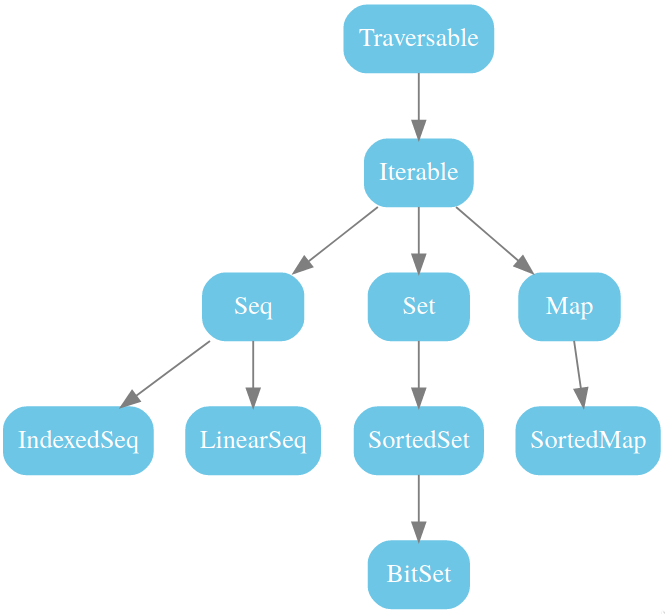
\includegraphics[width=1.0\textwidth]{../img/collection/collection-traits}
\end{Slide}
\noindent Läs mer om Scalas samlingar här: \\ 
\url{http://docs.scala-lang.org/overviews/collections/overview}


\begin{Slide}{Hierarki av samlingstyper i \texttt{scala.collection}}

\begin{multicols}{2}
\begin{tikzpicture}[sibling distance=6.1em,->,>=stealth', inner sep=3pt, %scale=0.5, 
  every node/.style = {shape=rectangle, draw, align=center,font=\small\ttfamily},
  class/.style = {fill=blue!20},
  trait/.style = {rounded corners, fill=red!20}]
  \node[trait] {Traversable}
    child { node[trait] {Iterable} 
      child { node[trait] {Seq} 
       }
      child { node[trait] {Set} 
      }
      child { node[trait] {Map} 
      }
    };
\end{tikzpicture}

\columnbreak
 
{\SlideFontTiny 

\code{Traversable} har metoder som är implementerade med hjälp av: \\
\code{def foreach[U](f: Elem => U): Unit}\\

\vspace{1em}\code{Iterable} har metoder som är implementerade med hjälp av: \\
\code{def iterator: Iterator[A] } 

}

\begin{itemize}\SlideFontTiny 
\item[] \code{Seq}: ordnade i sekvens
\item[] \code{Set}: unika element
\item[] \code{Map}: par av (nyckel, värde)
\end{itemize}


\end{multicols}

{\SlideFontSmall Samlingen \Emph{\texttt{Vector}} är en \code{Seq} som är en \code{Iterable} som är en \code{Traversable}.}
\end{Slide}

\begin{Slide}{Använda \texttt{iterator}}\SlideFontSmall
Med en \code{iterator} kan man \Emph{iterera} med \code{while} över alla element, men endast \Alert{en   gång}; sedan är iteratorn ''förbrukad''. (Men man kan be om en ny.)
\begin{REPL}
scala> val xs = Vector(1,2,3,4)
xs: scala.collection.immutable.Vector[Int] = Vector(1, 2, 3, 4)

scala> val it = xs.iterator
it: scala.collection.immutable.VectorIterator[Int] = non-empty iterator

scala> while (it.hasNext) print(it.next)
1234

scala> it.hasNext
res1: Boolean = false

scala> it.next
java.util.NoSuchElementException: reached iterator end
  at scala.collection.immutable.VectorIterator.next(Vector.scala:674)
\end{REPL}
\Emph{Normalt} behöver man \Alert{inte} använda \code{iterator}: det finns oftast färdiga metoder som gör det man vill, till exempel \code{foreach}, \code{map}, \code{sum}, \code{min} etc.
\end{Slide}

\begin{Slide}{Några användbara metoder på samlingar}\SlideFontTiny
\begin{tabular}{r r l}\hline
\texttt{\Emph{Traversable}} 
  & \code|xs.size| & antal elementet \\
  & \code|xs.head| & första elementet \\
  & \code|xs.last| & sista elementet \\
  & \code|xs.take(n)| & ny samling med de första n elementet \\
  & \code|xs.drop(n)| & ny samling utan de första n elementet \\
  & \code|xs.foreach(f)| & gör \code|f| på alla element, returtyp \code|Unit|\\
  & \code|xs.map(f)| & gör \code|f| på alla element, ger ny samling \\
  & \code|xs.filter(p)| & ny samling med bara de element där p är sant\\
  & \code|xs.groupBy(f)| & ger en \code|Map| som grupperar värdena enligt f\\ 
  & \code|xs.mkString(",")| & en kommaseparerad sträng med alla element\\ \hline
    
\texttt{\Emph{Iterable}} 
  & \code|xs.zip(ys)| & ny samling med par (x, y); ''zippa ihop'' xs och ys \\
  & \code|xs.zipWithIndex| & ger en \code|Map| med par (x, index för x) \\
  & \code|xs.sliding(n)| & ny samling av samlingar genom glidande ''fönster''\\ \hline

\texttt{\Emph{Seq}} 
  & \code|xs.length| & samma som \code|xs.size| \\
  & \code|xs :+ x| & ny samling med x sist efter xs \\
  & \code|x +: xs| & ny samling med x före xs \\ \hline
  
\end{tabular}

\pause
\vspace{0.5em}\Emph{Minnesregel} för \code{+:} och \code{:+  } \Alert{Colon on the collection side}

\pause
Prova fler samlingsmetoder ur snabbreferensen: ~~\url{http://cs.lth.se/quickref}
\end{Slide}



\begin{Slide}{Använda samlingsmetoder}
\begin{REPL}
scala> val tal = Vector(1,4,7,9,42)
tal: scala.collection.immutable.Vector[Int] = Vector(1, 4, 7, 9, 42)

scala> val jämna = tal.filter(_ % 2 == 0)
jämna: scala.collection.immutable.Vector[Int] = Vector(4, 42)

scala> val xs = Vector(("Kim","Smith"), ("Kim", "Jones"), ("Robin", "Smith"))
xs: scala.collection.immutable.Vector[(String, String)] = Vector((Kim,Smith), (Kim,Jones), (Robin,Smith))

scala> val grupperaEfterFörnamn = xs.groupBy(_._1)
grupperaEfterFörnamn: Map[String,Vector[(String, String)]] = 
Map(Kim -> Vector((Kim,Smith), (Kim,Jones)), Robin -> Vector((Robin,Smith)))

scala> val grupperaEfterEfternamn = xs.groupBy(_._2)
grupperaEfterEfternamn: Map[String,Vector[(String, String)]] = 
Map(Jones -> Vector((Kim,Jones)), Smith -> Vector((Kim,Smith), (Robin,Smith)))

\end{REPL}
\end{Slide}




\begin{Slide}{Mer specifik samlingstyper i \texttt{scala.collection}}
Det finns \Alert{mer specifika} \Emph{subtyper} av \code{Seq}, \code{Set} och \code{Map}:
\\ \vspace{1em}

\begin{tikzpicture}[sibling distance=5.8em,->,>=stealth', inner sep=3pt, %scale=0.5, 
  every node/.style = {shape=rectangle, draw, align=center,font=\small\ttfamily},
  class/.style = {fill=blue!20},
  trait/.style = {rounded corners, fill=red!20}]
  \node[trait] {Traversable}
    child { node[trait] {Iterable} 
      child { node[trait, xshift=-2.4cm] {Seq} 
        child { node[trait] {IndexedSeq} }
        child { node[trait] {LinearSeq} }
       }
      child { node[trait, yshift=-0.0cm] {Set} 
        child { node[trait] {SortedSet} }
        child { node[trait] {BitSet} }
      }
      child { node[trait, xshift=1.0cm] {Map} 
        child { node[trait] {SortedMap} }
      }
    };
\end{tikzpicture}

\vspace{0.5em}
\Emph{\texttt{Vector}} är en \Alert{\texttt{IndexedSeq}} medan
\Emph{\texttt{List}} är en \Alert{\texttt{LinearSeq}}.
\end{Slide}

\begin{Slide}{Några oföränderliga och förändringsbara sekvenssamlingar}\SlideFontSmall
\begin{tabular}{r l l}
\texttt{scala.collection.\Emph{immutable}.Seq.} & & \\
 & \code|IndexedSeq.| & \\
 & & \Emph{\texttt{Vector}} \\
 & & \Emph{\texttt{Range}} \\
 & \code|LinearSeq.| & \\
 & & \Emph{\texttt{List}} \\
   & & \Emph{\texttt{Queue}} \\

\texttt{scala.collection.\Alert{mutable}.Seq.} & & \\
 & \code|IndexedSeq.| & \\
 & & \Alert{\texttt{ArrayBuffer}} \\
 & & \Alert{\texttt{StringBuilder}} \\
 & \code|LinearSeq.| & \\
 & & \Alert{\texttt{ListBuffer}} \\
   & & \Alert{\texttt{Queue}} \\
\end{tabular}

Studera samlingars egenskaper här: \href{http://docs.scala-lang.org/overviews/collections/overview}{docs.scala-lang.org/overviews/collections/overview}
\end{Slide}


\begin{Slide}{scala.collection.immutable}
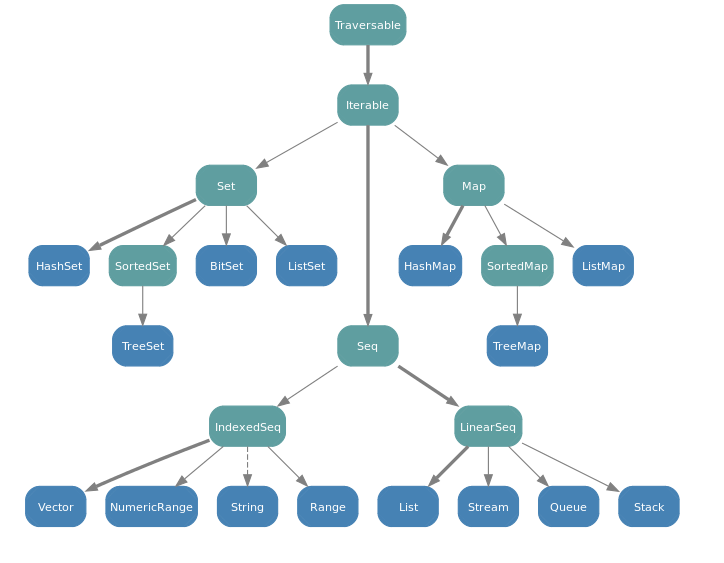
\includegraphics[width=0.82\textwidth]{../img/collection/collection-immutable}
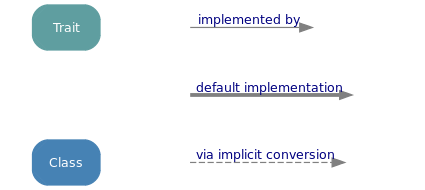
\includegraphics[width=0.33\textwidth]{../img/collection/collection-legend}
\end{Slide}


\begin{Slide}{scala.collection.mutable}
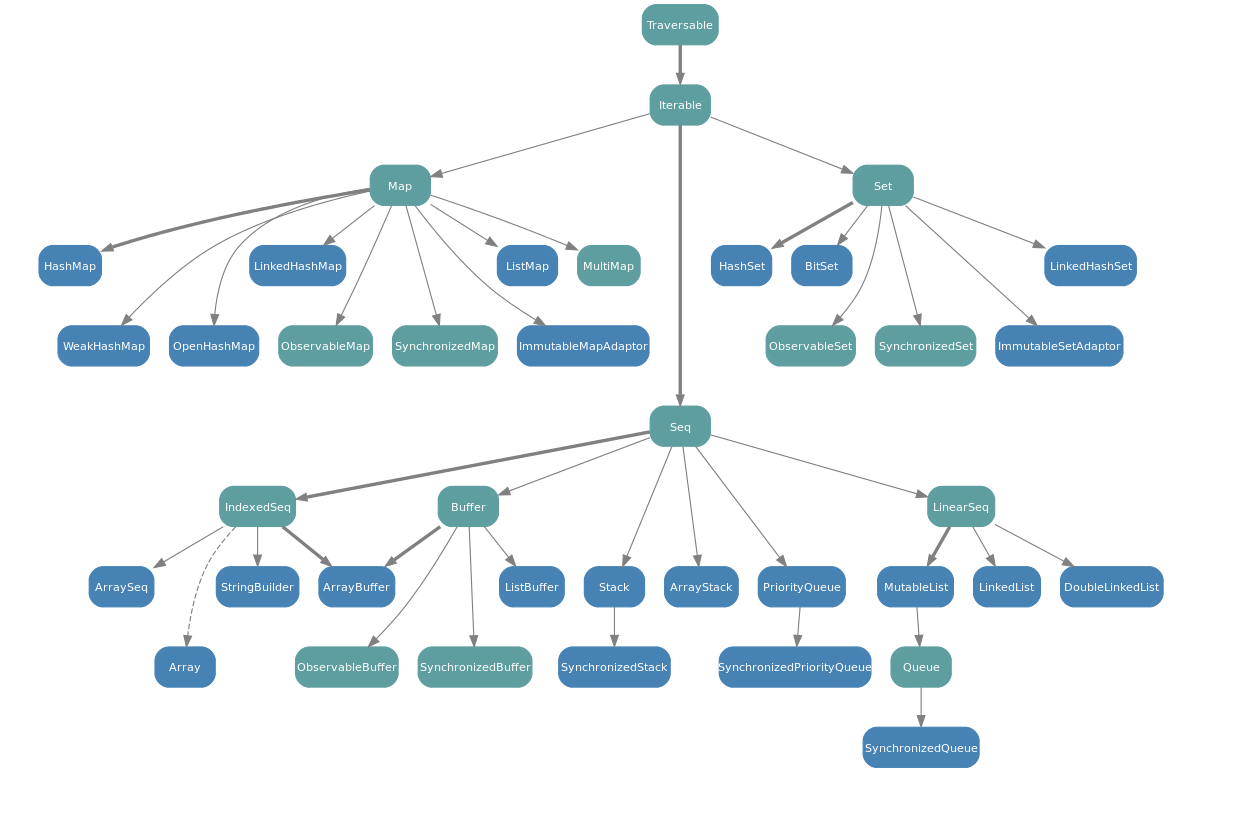
\includegraphics[width=1.05\textwidth]{../img/collection/collection-mutable}
\end{Slide}


\begin{Slide}{Strängar är implicit en \texttt{IndexedSeq[Char]}}\SlideFontSmall
Det finns en så kallad \Emph{implicit konvertering} mellan \code{String} och \code{IndexedSeq[Char]} vilket gör att \Alert{alla samlingsmetoder på \texttt{Seq} även funkar på strängar} och även flera andra smidiga strängmetoder erbjuds \Alert{utöver} de som finns i \href{http://docs.oracle.com/javase/8/docs/api/java/lang/String.html}{\code{java.lang.String}} genom klassen \href{http://www.scala-lang.org/api/current/#scala.collection.immutable.StringOps}{\code{StringOps}}.

\vspace{0.5em}
\begin{REPLnonum}
scala> "hej".  //tryck på TAB och se alla strängmetoder
\end{REPLnonum}
Detta är en stor fördel med Scala jämfört med många andra språk, som har strängar som inte kan allt som andra sekvenssamlingar kan.
\end{Slide}


\begin{Slide}{\texttt{Vector} eller \texttt{List}?}\SlideFontTiny
{\href{http://stackoverflow.com/questions/6928327/when-should-i-choose-vector-in-scala}{stackoverflow.com/questions/6928327/when-should-i-choose-vector-in-scala}}

\begin{enumerate}
\item If we only need to transform sequences by operations like map, filter, fold etc: basically it does not matter, we should program our algorithm generically and might even benefit from accepting parallel sequences. For sequential operations List is probably a bit faster. But you should benchmark it if you have to optimize.

\item If we need a lot of random access and different updates, so we should use vector, list will be prohibitively slow.

\item If we operate on lists in a classical functional way, building them by prepending and iterating by recursive decomposition: use list, vector will be slower by a factor 10-100 or more.

\item If we have an performance critical algorithm that is basically imperative and does a lot of random access on a list, something like in place quick-sort: use an imperative data structure, e.g. ArrayBuffer, locally and copy your data from and to it.
\end{enumerate}
{\href{http://stackoverflow.com/questions/20612729/how-does-scalas-vector-work}{stackoverflow.com/questions/20612729/how-does-scalas-vector-work}}\\
Mer om tids- och minneskomplexitet i fördjupningskursen och senare kurser.
\end{Slide}



\begin{Slide}{Mängd: snabb innehållstest, garanterat dubblettfri}\SlideFontSmall
En \Emph{mängd} \Eng{set} är en samling som \Alert{inte} kan innehålla \Alert{dubbletter} och som är snabb på att avgöra om ett element \Alert{finns eller inte} i mängden.

\begin{REPL}
scala> var veg = Set.empty[String]
veg: scala.collection.immutable.Set[String] = Set()

scala> veg = veg + "Gurka"
veg: scala.collection.immutable.Set[String] = Set(Gurka)

scala> veg = veg ++ Set("Broccoli", "Tomat", "Gurka")
veg: scala.collection.immutable.Set[String] = Set(Gurka, Broccoli, Tomat)

scala> veg.contains("Gurka")
res0: Boolean = true

scala> veg.apply("Gurka")   // samma som contains
res1: Boolean = true

scala> veg("Morot")
res2: Boolean = false
\end{REPL}

\end{Slide}

\begin{Slide}{Den fantastiska nyckel-värde-tabellen \texttt{Map}}\SlideFontSmall
\begin{itemize}
\item En \Emph{nyckel-värde-tabell} \Eng{key-value table} är en slags generaliserad vektor där man kan ''indexera'' med godtycklig typ. 

\item Kallas öven \href{https://sv.wikipedia.org/wiki/Hashtabell}{\Emph{hashtabell}} \Eng{hash table}, \Emph{lexikon} \Eng{dictionary} eller kort och gott \Emph{mapp} \Eng{map},

\item En hashtabell är en \Emph{samling av par}, där varje par består av en \Alert{unik} \Emph{nyckel} och ett tillhörande \Emph{värde}. 

\item Om man vet nyckeln kan man få fram värdet \Alert{snabbt}, på liknande sätt som indexering sker i en vektor om man vet heltalsindex. 

\item Denna datastruktur är \Alert{mycket användbar} och liknar en enkel databas.
\end{itemize}
\begin{REPL}
scala> val födelse = Map("C" -> 1972,  "C++" -> 1983, "C#" -> 2000, 
  "Scala" -> 2004, "Java" -> 1995, "Javascript" -> 1995, "Python" -> 1991)

födelse: scala.collection.immutable.Map[String,Int] = Map(Scala -> 2004, C# -> 2000, Python -> 1991, Javascript -> 1995, C -> 1972, C++ -> 1983, Java -> 1995)
  
scala> födelse.apply("Scala")
res0: Int = 2004

scala> födelse("Java")
res1: Int = 1995

\end{REPL}
\end{Slide}

\begin{Slide}{Exempel nyckel-värde-tabell}
\begin{REPL}
scala> val färg = Map("gurka" -> "grön", "tomat"->"röd", "aubergine"->"lila")
färg: scala.collection.immutable.Map[String,String] = 
  Map(gurka -> grön, tomat -> röd, aubergine -> lila)

scala> färg("gurka")
res0: String = grön

scala> färg.keySet
res1: scala.collection.immutable.Set[String] = Set(gurka, tomat, aubergine)

scala> val ärGrönSak = färg.map(elem => (elem._1, elem._2 == "grön"))
ärGrönSak: Map[String,Boolean] = Map(gurka -> true, tomat -> false, aubergine -> false)

scala> val baklängesFärg = färg.mapValues(s => s.reverse)
baklängesFärg: Map[String,String] = Map(gurka -> nörg, tomat -> dör, aubergine -> alil)

\end{REPL}
\begin{itemize}
\item \code{xs.keySet} ger en mängd av alla nycklar
\item \code{xs.map(f)} mappar funktionen f på alla par av (key, value)
\item \code{xs.mapValues(f)} mappar funktionen f på alla värden 
\end{itemize}

\end{Slide}

\begin{Slide}{Metoderna zipWithIndex, groupBy och mapValues}
\begin{REPL}
scala> val högaKort = Vector("Knekt", "Dam", "Kung", "Äss")

scala> val kortIndex = högaKort.zipWithIndex.toMap
kortIndex: Map[String,Int] = Map(Knekt -> 0, Dam -> 1, Kung -> 2, Äss -> 3)

scala> kortIndex("Kung") > kortIndex("Knekt") 
res0: Boolean = true

scala> val xs = Vector(("Kim","Smith"), ("Kim", "Jones"), ("Robin", "Smith"))
xs: Vector[(String, String)] = Vector((Kim,Smith), (Kim,Jones), (Robin,Smith))

scala> val grupperaEfterFörnamn = xs.groupBy(_._1)
grupperaEfterFörnamn: Map[String,Vector[(String, String)]] = 
Map(Kim -> Vector((Kim,Smith), (Kim,Jones)), Robin -> Vector((Robin,Smith)))

scala> val grupperaEfterEfternamn = xs.groupBy(_._2)
grupperaEfterEfternamn: Map[String,Vector[(String, String)]] = 
Map(Jones -> Vector((Kim,Jones)), Smith -> Vector((Kim,Smith), (Robin,Smith)))

scala> val frekvens = xs.groupBy(_._1).mapValues(_.size)
frekvens: Map[String,Int] = Map(Kim -> 2, Robin -> 1)
\end{REPL}
\end{Slide}


\begin{Slide}{Speciella metoder på förändringsbara samlingar}\SlideFontSmall
Både \code{Set} och \code{Map} finns i \Alert{förändringsbara} varianter med extra metoder för uppdatering av innehållet ''på plats'' utan att nya samlingar skapas.
\begin{REPL}
scala> import scala.collection.mutable

scala> val ms = mutable.Set.empty[Int]
ms: scala.collection.mutable.Set[Int] = Set()

scala> ms += 42
res0: ms.type = Set(42)

scala> ms += (1, 2, 3, 1, 2, 3); ms -= 1
res1: ms.type = Set(2, 42, 3)

scala> ms.mkString("Mängd: ", ", ", s" Antal: ${ms.size}")
res2: String = Mängd: 1, 2, 42, 3 Antal: 4

scala> val ordpar = mutable.Map.empty[String, String]
scala> ordpar += ("hej" -> "svejs", "abra" -> "kadabra", "ada" -> "lovelace")
scala> println(ordpar("abra"))
kadabra
\end{REPL}
\end{Slide}

\begin{Slide}{Fler exempel på samlingsmetoder}
Exempel: räkna bokstäver i ord.  \\
Undersök vad som händer i REPL:
\begin{Code}[basicstyle=\SlideFontSize{9}{13}\ttfamily]
val ord = "sex laxar i en laxask sju sjösjuka sjömän" 
val uppdelad = ord.split(' ').toVector
val ordlängd = uppdelad.map(_.length)
val ordlängdMap = uppdelad.map(s => (s, s.size)).toMap
val grupperaEfterFörstaBokstav = uppdelad.groupBy(s => s(0))
val bokstäver = ord.toVector.filter(_ != ' ')
val antalX = bokstäver.count(_ == 'x')
val grupperade = bokstäver.groupBy(ch => ch)
val antal = grupperade.map(kv => (kv._1, kv._2.size))
val sorterat = antal.toVector.sortBy(_._2)
val vanligast = antal.maxBy(_._2)
\end{Code}
\end{Slide}


\begin{Slide}{Jobba med föränderlig samling lokalt; \\ returnera oföränderlig samling när du är klar}
\SlideFontSmall
Om du vill implementera en imperativ algoritm med en föränderlig samling:\\ 
Gör gärna detta \Alert{lokalt} i en \Alert{förändringsbar} samling och returnera sedan en \Emph{oföränderlig} samling, genom att köra t.ex. \code{toSet} på en mängd, eller \code{toMap} på en hashtabell, eller \code{toVector} på en \code{ArrayBuffer} eller \code{Array}.

\begin{REPL}
scala> :paste
def kastaTärningTillsAllaUtfallUtomEtt(sidor: Int = 6) = {
  val s = scala.collection.mutable.Set.empty[Int]
  var n = 0
  while (s.size < sidor - 1) {
    s += (math.random * sidor + 1).toInt
    n += 1
  }
  (n, s.toSet)
}
scala> kastaTärningTillsAllaUtfallUtomEtt()
res0: (Int, scala.collection.immutable.Set[Int]) = (13,Set(5, 1, 6, 2, 3))

\end{REPL}

\end{Slide}






%!TEX encoding = UTF-8 Unicode
%!TEX root = ../lect-w07.tex


\Subsection{Läsa från fil och URL}

\begin{Slide}{Serialisering och deserialisering}
\begin{itemize}
  \item Att \Emph{serialisera} innebär att \Alert{koda objekt} i minnet till en avkodningsbar \Alert{sekvens av symboler}, som kan lagras t.ex. i en fil på din hårddisk.
  \item Att \Emph{de-serialisera} innebär att \Alert{avkoda en sekvens av symboler}, t.ex. från en fil, och \Alert{återskapa objekt} i minnet.
\end{itemize}
\end{Slide}


\begin{Slide}{Läsa från fil och URL}
I paketet \code{scala.io} finns singelobjektet \code{Source} med metoderna \code{fromFile} och \code{fromUrl} för läsning från fil resp. från  URL\footnote{URL = Universal Resource Locator}, som börjar t.ex. med \code{http://}
\begin{Code}
def läsFrånFil(filnamn: String) = scala.io.Source.fromFile(filnamn).mkString

def läsRaderFrånFil(filnamn: String): Vector[String] =
  scala.io.Source.fromFile(filnamn).getLines.toVector

def läsFrånWebbsida(url: String) = scala.io.Source.fromFile(url).mkString

def läsRaderWebbsida(url: String, kodning: String = "UTF-8"): Vector[String] =
  scala.io.Source.fromFile(url, kodning).getLines.toVector

\end{Code}
Se exempel på veckans övning.
\end{Slide}


\begin{Slide}{Fördjupning: singelobjektet Disk}
Se fördjupningsuppgift övning \texttt{lookup}:
\scalainputlisting[basicstyle=\ttfamily\SlideFontSize{6}{7.5}]{../compendium/examples/Disk.scala}
\end{Slide}

%!TEX encoding = UTF-8 Unicode
%!TEX root = ../lect-w07.tex

\ifkompendium\else
\Subsection{Grumligtlådan}

\begin{Slide}{Grumligtlådan: topplista med ämnen}
\begin{multicols}{2}
\begin{verbatim}
  om kursen       : 14
  klass           : 9
  this            : 7
  filstruktur     : 5
  pluggteknik     : 4
  case-klass      : 4
  registrera      : 3
  filtrera        : 3
  copy            : 3
  tupel           : 2
  konstruktor     : 2
  iterera         : 2
  fabriksmetod    : 2
  synlighet       : 1
  skuggning       : 1
  sidoeffekt      : 1
  Seq[T]          : 1
  sekvenser       : 1
  sats/uttryck    : 1
  lambda          : 1
  kompanjonsobj   : 1
  högre ordn funk : 1
  funktion        : 1
  curry-funktion  : 1
\end{verbatim}
\end{multicols}
\end{Slide}



\begin{Slide}{Grumligtlådan: lajvkodning}
Lajvkodning enligt begrepp i lådan utifrån denna klass:
\begin{Code}[basicstyle=\ttfamily\SlideFontSize{12}{14}]
class Frog(var n: Int) { def hop = n += 1 }
\end{Code}

\includegraphics[width=0.6\textwidth]{../img/frog}
\end{Slide}

\fi


\end{document}
